\section{Estimation}

\subsection{Time-series cross validation}

Sections \ref{sec:best-subset-mip} and \ref{sec:best-subset-ell1} presented two different methods to estimate the conditional distribution in a parsimonious way. However, as presented, the aforementioned methods don't provide a unique solution, but a set of solutions for a range of tuning parameters. For instance, on the MILP method, the quantity $K$ of nonzero coefficients is an input of the problem. Similarly, the LASSO needs a penalization parameter $\lambda$, that tunes how much penalty the $\ell_1$-norm receives.

In statistics and machine learning, a popular technique is using Cross-validation (CV) to select the best model from this range of possibilities.
It is a technique used to have an estimative of the model's quality of prediction in an independent testing set. The best model that minimizes the CV error is the model which presumably will have the best performance on out of sample data.

The usage of CV is not straightforward when data is dependent, which is the case when working with time series. As the data is time dependent, one can be interested in using either all observations or to take the dependency away. The works
\cite{bergmeir_note_2017} and \cite{bergmeir_use_2012} deals specifically with the usage of CV in a time series context. They provide tests with both $K$-fold CV and $K$-fold with non-dependent data. Both schemes are shown of Figure \ref{fig:cross-validation-scheme}.
This mimics real applications better even by dropping in a few times the number of observations. Will use a growing window in a 5-fold scheme.
\begin{figure}
	\centering
	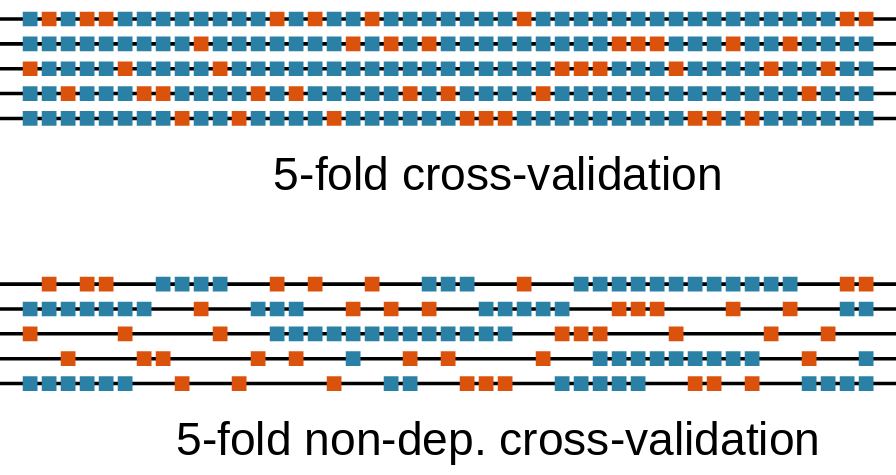
\includegraphics[width=0.9\linewidth]{Figuras/Cross-validation-scheme}
	\caption{$K$-fold CV and $K$-fold with non-dependent data. Observations in blue are used to estimation and in orange for evaluation. Note that non-dependent data doesn't use all dataset in each fold.}
	\label{fig:cross-validation-scheme}
\end{figure}
In both settings, the training data is randomly split into a collection of sets $J_k$, forming a $K$ size partition. Each of these $J_k$ is used as test set, while \todoi{terminar parágrafo de explicação sobre CV}

% \todoi{Ver se novas figuras (R/grafico-cv.r) e ver se incluir outras formas de CV} % escolhemos trabalhar apenas com este tipo de CV



\subsection{Information Criteria for Quantile Regression}
Sometimes, using CV can be computationally expensive, as the full estimation is done several times for each tuning parameter - in this case, either $K$ or $\lambda$. Other form of deciding the quantity of variables that provides a good equilibrium between in-sample prediction and parsimony is the Information Criteria.

Information criteria summarizes two aspects. One of them refers to how well the model fits the in-sample observations and the other part penalizes the quantity of covariates used in the model. By penalizing how big our model is, we prevent overfitting from happening. So, in order for a covariate to be included in the model, it must supply enough goodness of fit.
In \cite{machado1993robust}, it is presented a variation of the Schwarz criteria for M-estimators that includes quantile regression. The Schwarz Information Criteria (SIC), adapted to the quantile autoregression case, is presented below:
\begin{align} 
\begin{split}
SIC(m) = n \log({obj}^*)+\frac{1}{2}K\log n,\label{eq:SIC}
\end{split}					
\end{align}
where $K$ is the model's dimension. This procedure leads to a consistent model selection if the model is well specified. 

By minimizing the $SIC$ \todoi{acabar}

\subsection{Model selection distance}
%
%On sections \ref{sec:best-subset-mip} and \ref{sec:best-subset-ell1}, we presented two ways of selecting variables. Nonetheless, regularization can be done with different levels of parsimony. For example, one can select a different number $K$ of variables to be included in the best subset selection via MILP or choose different values of $\lambda$ for the $\ell_1$ penalty. 
%There is a tradeoff between variability and bias, when selecting the number of variables in a model. In order to  

% % % Métrica

Solving a LP problem such as the LASSO is many times faster than a similar-sized MILP problem, for introducing binary variables breaks the problem's convexity. On the other hand, in our case the MILP solution is the exact best solution in minimizing the QR objective function, while the LASSO is an approximation of that.

One of our goals is to test how far from the optimal solution is the LASSO.
%It would be interesting, then, to use a faster method that would provide a solution close to the optimal. 
%To test how far are the solutions given by both methods, we propose an experiment that is described as follows. 
For each number $K$ of total nonzero coefficients, there will be a penalty $\lambda^*_K$ which minimizes the errors from the quantile regression's objective function (given on equation (\ref{eq:post-lasso})): 
%\todo{($K$ ranging from 0 until 12, where 0 means that only the intercept is included)}
\begin{equation}
\lambda^*_K = \argmin_\lambda \left\lbrace \left.  obj_{\lambda}^{*} \quad  \right| \, \| \beta^*_\lambda \|_0 = K \right\rbrace,
\end{equation}
where the quantity $\| \beta^*_\lambda \|_0$ is the $0$-norm, which gives the total of nonzero coefficients, for a given lambda of the LASSO estimations.

We, then, define the sets $L_K^{LASSO}$ and $L_K^{MILP}$, which contains all nonzero indexes, for a given $K$, when using methods LASSO and MILP for regularization, respectively.
Thus, we can compare the best LASSO fit where exactly $K$ variables are selected with the best fit given by the MILP problem, also with $K$ variables selected.

As the MILP solution is the exact solution for the problem, while the LASSO solution is an approximation, we use the former as a \textit{benchmarking} for the quality of the latter solution. It is desirable that the LASSO solution be as related with the MILP solution as possible. The difference in performance is given by a similarity metric $d$, which measures distance from solutions weighted by the correlation between variables. 
The similarity is calculated as the solution of the following optimization problem
\begin{IEEEeqnarray}{lC}
	d(\beta^*_{MILP(K)}, \beta^*_{\lambda^*_K}) = \min_{0\leq\delta_{ij}\leq1} & \sum\limits_{i,j = 1}^K  \delta_{ij} (1-|\rho_{ij}|) \label{eq:metricad0} \\
	\text{subject to} & \nonumber \\
	\sum\limits_{j =1}^K\delta_{ij}=1, &  i=1,\dots,K,\\
	\sum\limits_{i =1}^K\delta_{ij}=1, & j=1,\dots,K,
\end{IEEEeqnarray}
where $\rho_{ij}$ is the correlation between the $i$-th and $j$-th independent variables in sets $L_k^{MILP}$ and $L_k^{LASSO}$, respectively. The optimal value for the decision variables of this problem provides us with an assignment between selected covariates from both methods, namely, MILP and LASSO, that minimizes the overall ``index of uncorrelation" between selected covariates. If $\delta^*_{ij} = 1$, the $i$-th selected variable in  $L_k^{MILP}$ is associated with the $j$-th variable  in $L_k^{LASSO}$. For instance, if $d(\beta^*_{MILP(K)}, \beta^*_{\lambda^*_K}) = 0$, it means that there are $K$ perfectly correlated pair of variables, even though not being the same subset. 


\subsection{Evaluation criteria}
The full dataset is split between the test set - which evaluates our methodology's forecasting performance - and the training set - which we use to estimate parameters.  This setting mimics real world applications, where the future is unknown.

As conditional distribution is the focus in this paper, we use a performance measurement which emphasizes the correctness of each quantile. 
For each observation $y_t$ and probability $\alpha \in A$, a score function
is defined by

\[
L(A)= \sum_{t\in T}\rho_{\alpha}(y_{t}-q_{\alpha}(x_t))
\]
The error measure is defined as the average of the score function
for all observations and target quantiles.


% % % Trocar o sigma da função objetivo.




% % % recolocar no texto





